\chapter{Agent training and experiments in ideal simulation environment}
Chapters 4 and 5 focus on the experimental phase of the project. This chapter details the training procedure of our SAC agent for the swing-up task and then transitions to a simulation phase to validate results for both the swing-up and stabilization tasks. We have structured this chapter into three distinct subsections: training setup, training process, and simulation results.

The first subsection describes the foundation of a reinforcement learning interaction rooted in a stable baseline3-based RL algorithm. It also touches upon a customized environment inherited from the OpenAI Gym environment. The second subsection centers on hyperparameter tuning and highlights the challenges encountered during training. The third subsection displays the results acquired from both the pendubot and acrobot setups.

\section{Ideal training setup}
Stable Baseline 3(SB3)\cite{stable-baselines3} is an open-source implementation of deep reinforcement learning algorithms based on the Python language. This library includes seven commonly used model-free deep reinforcement learning algorithms including SAC. Prior implementations of deep RL algorithms often encountered a problem wherein small implementation details could greatly affect performance, typically exceeding the differences between algorithms\cite{islam2017reproducibility}. The developers of SB3 have done a commendable job stabilizing the performance of these deep RL algorithms by benchmarking each one on common environments and comparing them to prior implementations. Owing to its user-friendly and reliable nature, we chose Stable Baseline 3 as our RL library, which greatly simplified our research process.

OpenAI Gymnasium\cite{towers_gymnasium_2023} is a toolkit for developing and comparing reinforcement learning algorithms, and it is widely used in the research community. Among its many advantages are its open-source nature and standardized environments, which facilitate the rapid testing and benchmarking of new algorithms. Additionally, it offers easy visualization and monitoring. Our decision to use the Gymnasium library is based on its extensibility—from standard environments to highly customized ones—as well as its capability to integrate with tools like PyTorch and TensorFlow for GPU-accelerated computations. Furthermore, Gymnasium provides the ability to construct stacked training environments for parallel training.

\begin{figure}[htbp]
    \centering
    
\includegraphics[width=0.8\linewidth]{figures/simulation_result/RL_interaction.png}
    \caption{Interaction between reinforcement learning agent and customized environment}
    \label{fig:RL_interaction}
\end{figure}

To construct the customized environment, we begin with the dynamic function that captures the nonlinear dynamics of the underactuated double pendulum from this respository\cite{2023_ram_wiebe_double_pendulum}. The dynamic function uses the current state observation and the action determined by the control policy, producing the next state via a Runge-Kutta integrator.

This integrated state is then input into the reward function, which yields a scalar output. This output is subsequently relayed to the SAC algorithm for policy evaluation and update. After these computations, the simulation calculates the current state, and the policy identifies the most probable action. Both of these values are then directed back to the dynamics function, initiating a new cycle.

It is widely recognized in the field of reinforcement learning that algorithms tend to converge more effectively when utilizing normalized state and action spaces \cite{sutton2018reinforcement}. Therefore, a scaling mechanism is designed to map the state and action spaces from their normalized versions to real-world measurements. The activation or deactivation of this scaling is optional.

For instance, in the case of a normalized state within the interval $[-1,1]$, we may choose to map it to real-world measurements such as $p_1$ in $[0,2\pi]$, $p_2$ in $[-\pi,\pi]$, and velocities $v_1$ and $v_2$ in $[-20,20]$ rad/s, while maintaining torque within the range $[-\tau_{\text{limit}}, \tau_{\text{limit}}]$. When this scaling mechanism is activated, it ensures that states and actions within the SAC algorithm always remain within the $[-1,1]$ boundary, thereby often leading to faster convergence.

The logic of the pipeline of the interaction of customized environment is described in the picture below.

\begin{figure}[H]
    \centering
    
\includegraphics[width=0.85\linewidth]{figures/simulation_result/scaling_mechanism.png}
    \caption{Detailed scaling pipeline in training process}
    \label{fig:scasling_mech}
\end{figure}

Previous work in the double pendulum repository has featured several combinations of link lengths, designated as designs A, B, C, and D. Each design has undergone various system identification attempts, resulting in different outcomes labeled as models 1.0, 2.0, and so on. The combinations of these designs are displayed below:

\begin{table}[ht]
\centering
\begin{tabular}{|c|c|c|c|c|}
\hline
  & design A & design B & design C & design D \\
\hline
$l_1$(m) & 0.3 & 0.3 & 0.2 & 0.3 \\
\hline
$l_2$(m) & 0.2 & 0.4 & 0.3 & 0.3 \\
\hline
\end{tabular}
\caption{Combinations of $l_1$ and $l_2$ of different designs}
\label{tab:different_designs}
\end{table}

In addition, the trial phase during training introduces a noisy initialization by adding Gaussian noise to the presumed initial state \([0,0,0,0]^T\), thereby increasing exploration. The mean of this Gaussian noise is set to \([0,0,0,0]^T\), and the covariance matrix is diagonal, specified as \(diag(0.01,0.01,0.005,0.005) \). For the evaluation phase, a zero initialization is employed to ensure the exploitation of the learned policy.

\section{Ideal training process}
During the training of the SAC controller for both the acrobot and pendubot, the primary focus was on tuning several key hyperparameters. These encompassed the learning rate, control frequency, episode length, and learning timestep. Effort was invested in adjusting hyperparameters for the reward function and the LQR controller, given their pivotal roles in the learning process, as detailed in Table \ref{tab:training_parameters}.

The learning rate was set at 0.01 to promote effective learning and adaptation. Additionally, the control frequency during training was configured to 100Hz, ensuring frequent updates and heightened responsiveness in the control process. An episode length of 1000 was selected for both the Acrobot and Pendubot, translating to 10-second-long episodes, to provide sufficient exploration and learning opportunities. To harness the full training potential, a total of 2e7 learning time steps were executed for the pendubot and 5e7 for the acrobot, allowing the agent to accumulate vast experience and enhance its performance.

\begin{table}[H]
  \centering
  \begin{tabular}{p{2cm} | p{3cm} | p{3cm} | p{3cm}}
  Robot & Quadratic Reward  & Constant Reward & LQR\\
  \hline
  \multirow{5}{*}{Pendubot} & \(Q_1\) = 8.0  &  & \(Q_1\) = 1.92\\
  & \(Q_2\) = 5.0  & \(r_{line}=500\) & \(Q_2\) = 1.92\\
  & \(Q_3\) = 0.1  & \(r_{vel}=0.0\) & \(Q_3\) = 0.3\\
  & \(Q_4\) = 0.1  & \(r_{LQR}=1e4\)& \(Q_4\) = 0.3\\
  & \(R\) = 1e-4  & & \(R\) = 0.82\\
  \hline
  \multirow{5}{*}{Acrobot} & \(Q_1\) = 10.0  &  & \(Q_1\) = 0.97\\
  & \(Q_2\) = 10.0  & \(r_{line}=500\) & \(Q_2\) = 0.93\\
  & \(Q_3\) = 0.2  & \(r_{vel}=1e4\) & \(Q_3\) = 0.39\\
  & \(Q_4\) = 0.2  & \(r_{LQR}=1e4\) & \(Q_4\) = 0.26\\
  & \(R\) = 1e-4  &  & \(R\) = 0.11\\
  \end{tabular}
 \caption{Hyper parameters used for the SAC training and the LQR controller.[may change]}
 \label{tab:training_parameters}
\end{table}

One of the successful learning curves for a total of 2e7 timesteps for the pendubot is illustrated below. This experiment, like all other simulation experiments done on the pendubot setup, uses design A, namely, $l_1 = 0.3m$ and $l_2 = 0.2m$. As depicted in the figure, from 0 to 1e7 timesteps, the learning curve experiences a gradual ascent. Between 1e7 and 1.2e7 timesteps, the learning curve surges rapidly, peaking at around one million in reward. After 1.2e6 timesteps, the curve begins to stabilize with occasional fluctuations, and no substantial increase in reward is observed.

\begin{figure}[H]
    \centering
    \fbox{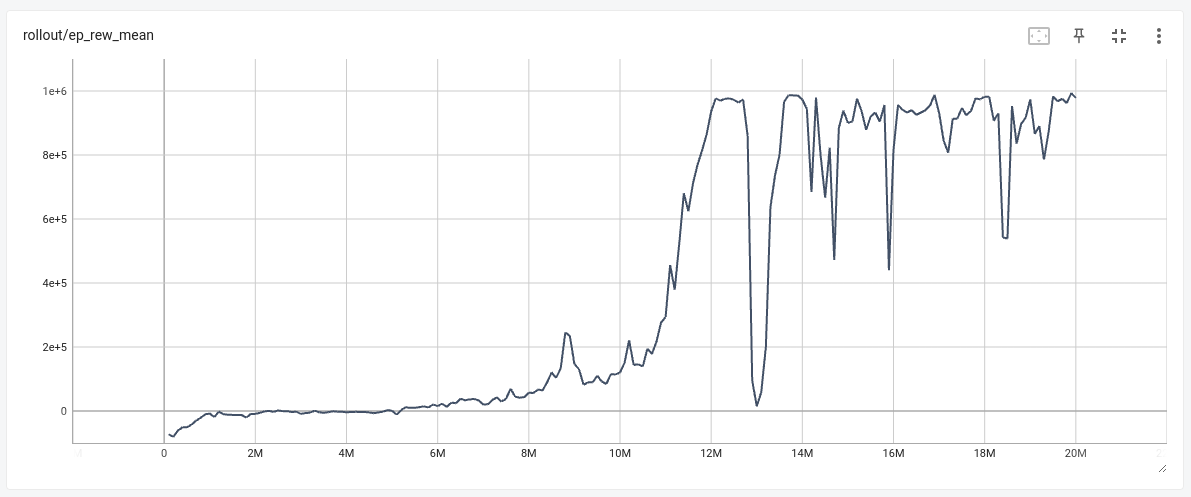
\includegraphics[width=1.0\textwidth]{figures/learning_curve/pendubot_learning_curve.png}} % First image
    \caption{Pendubot learning curve}
    \label{fig:image_a}
\end{figure}

The training on the acrobot are based on design C, with $l_1$ being 0.2m and $l_2$ being 0.3m. As shown in the successful learning curve over a total of 3e7 timesteps for the acrobot, the curve experienced relatively steady growth until 1.8e7 timesteps. After a sudden drop in reward between 1.8e7 and 2e7 timesteps, the learning curve began to increase drastically, with two major setbacks. By 3e7 timesteps, the learning curve had not reached its peak. We extended the learning period to 5e7 using a warm start from the model obtained at 3e7 timesteps, and the learning curve began to stabilize around 4e7 time steps.

\begin{figure}[H]
    \centering
    \fbox{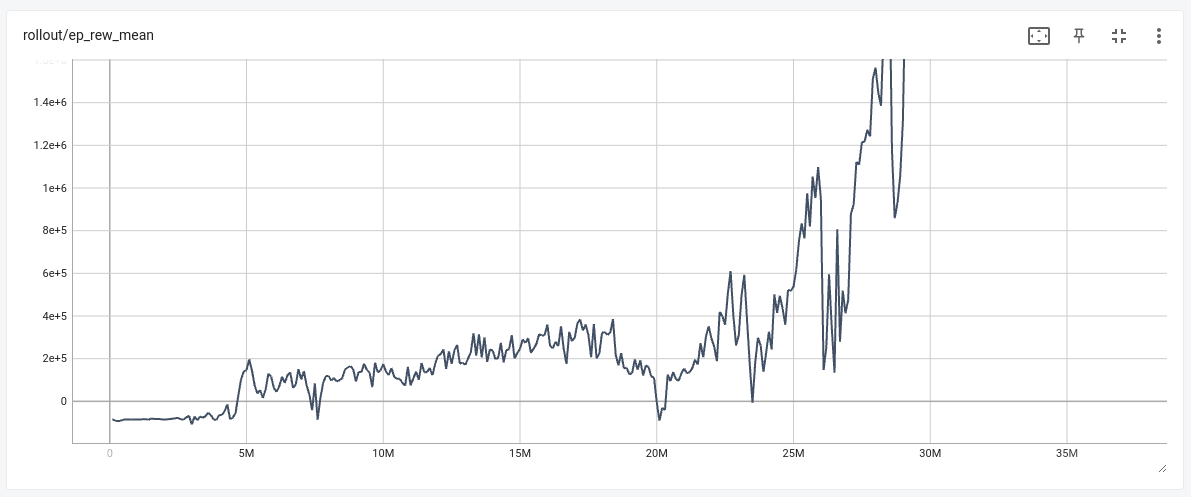
\includegraphics[width=1.0\textwidth]{figures/learning_curve/acrobot_learning_curve.png}} % Second image
    \caption{Acrobot learning curve}
    \label{fig:image_b}
\end{figure}

% In conclusion, the training for the pendubot converges more quickly than that for the acrobot. Additionally, based on the training curves, the pendubot's training process is more stable than the acrobot's.

\section{Ideal simulation results}
In this section, the simulation results for the acrobot and pendubot are presented separately. The model trained using the SAC algorithm is utilized during the swing-up stage and switches to the LQR controller when nearing the upright position. The primary success criteria for both swing-up and stabilization involve swinging up the double pendulum and maintaining its stability around the upright position for a prolonged period. Therefore, a total simulation time of 10 seconds is used. If the double pendulum fails to swing up within these 10 seconds, the result is deemed unsuccessful. Similarly, if the double pendulum loses stability within this time frame, the outcome is still considered a failure.

\subsection{Pendubot simulation in ideal environment}
The testing environment, identical to the customized learning environment employed during the evaluation phase in training, has been established to validate the training outcomes and replicate the agent's learned behavior from the reinforcement learning process. This testing environment is considered ideal as it excludes disturbances such as friction and damping, focusing solely on the effects of gravity, joint torque, and mechanical constraints. In this environment, zero initialization is applied instead of the noisy initialization. The system begins with an initial state of \([0,0,0,0]^T\), representing its lowest point with zero velocity, and initiates the swing-up using the control policy exclusively derived from SAC.

As depicted in the figure, the swing-up time is under 1 second. After this, the state of the pendubot enters the Region of Attraction (ROA) of the LQR controller. The transition between the two controllers is both seamless and effective, with the system stabilizing towards the desired state under the LQR controller's influence. This validates the effectiveness of the ROA method for the LQR takeover.

A significant highlight from this successful simulation is the impressively short swing-up time, despite having strict torque limit in place. However, a concerning feature observed from this simulation is the noisiness of the input control signal. The torque alternates signs rapidly, and the gradient of the torque tends to have a high absolute value.

\begin{figure}[H]
    \centering
    \fbox{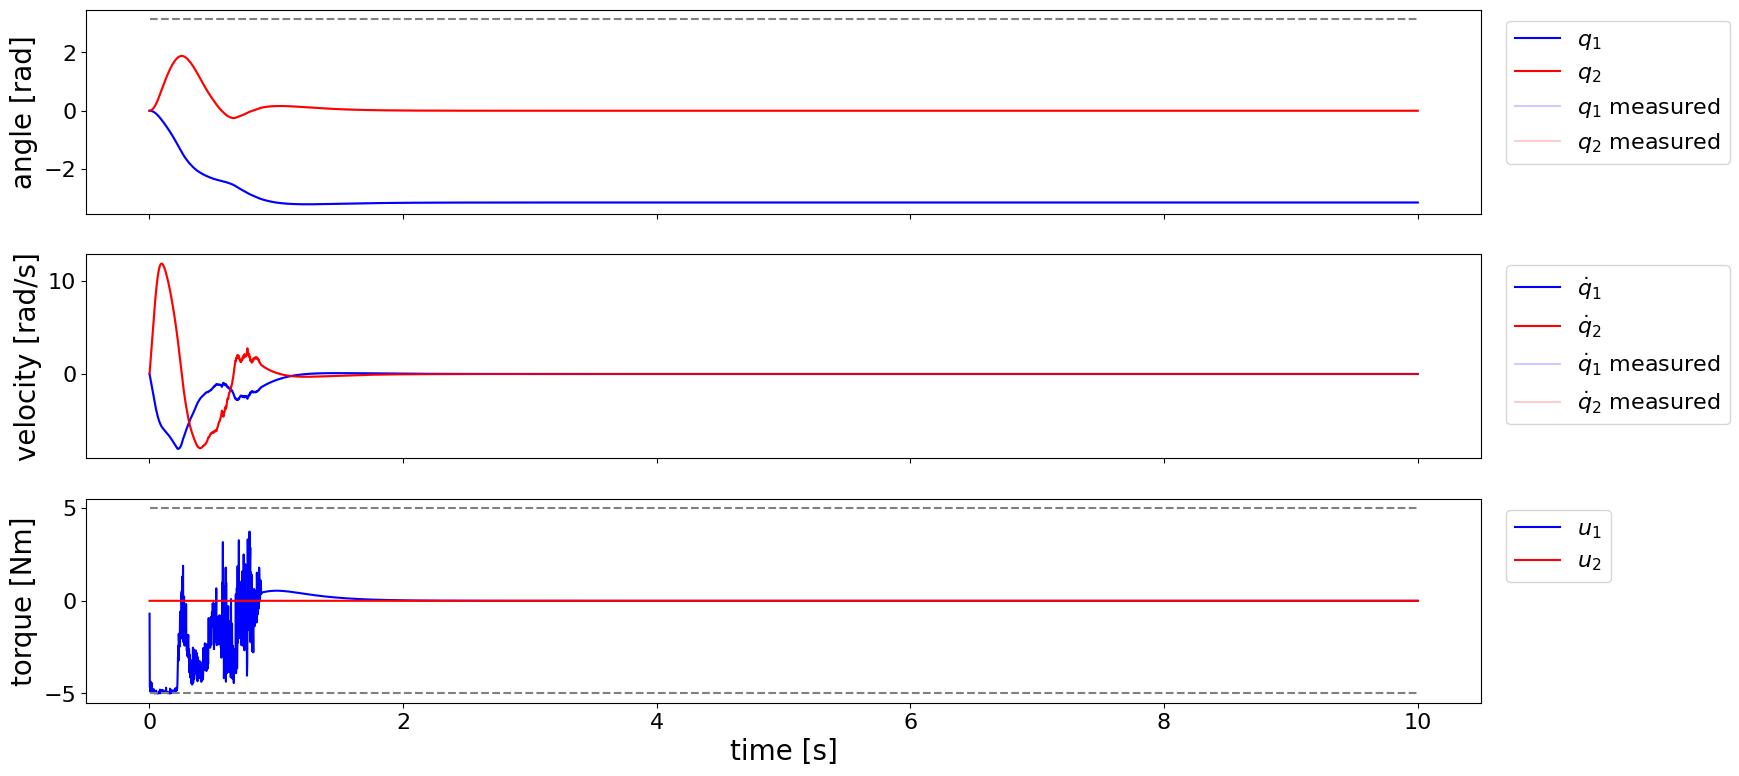
\includegraphics[width=0.9\textwidth]{figures/simulation_result/pendubot_unclipped.png}} % First image
    \caption{Pendubot simulation result}
    \label{fig:ideal_simulation_pendubot}
\end{figure}

\subsection{Acrobot simulation in ideal environment}

Just like the pendubot simulation, experiments on the acrobot setup are conducted in an ideal environment identical to the evaluation environment during the training phase. The acrobot begins its swing from the downward position with zero velocity, with the final goal of stabilizing around its highest point.

The accompanying image depicts a successful swing-up and stabilization within a 10-second window. The swing-up process takes about 2 seconds before the LQR effectively assumes control, maintaining an asymptotic stability around the target state with minimal fluctuations.

\begin{figure}[H]
    \centering
    \fbox{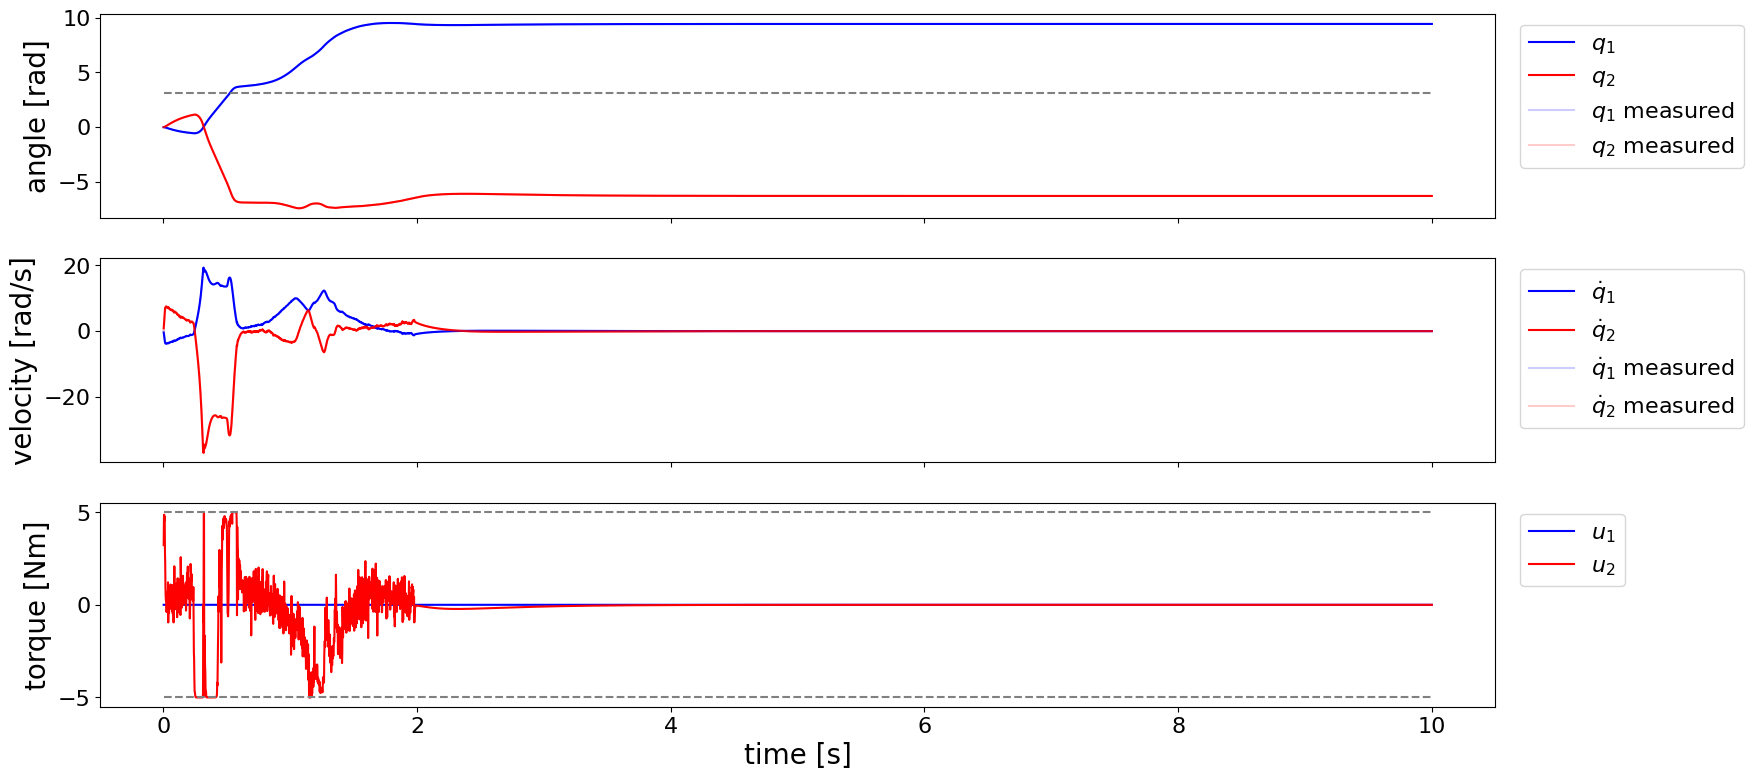
\includegraphics[width=0.9\textwidth]{figures/simulation_result/acrobot_unclipped.png}} % Second image
    \caption{Acrobot simulation result}
    \label{fig:ideal_simulation_acrobot}
\end{figure}

In comparison to the pendubot's simulation curves, the swing-up time for the acrobot is roughly twice as long. This aligns with the notion that controlling the acrobot is a more challenging task than the pendubot. A shared drawback observed in both simulations is the lack of torque smoothness. For the acrobot, the input torque exhibits several significant jumps from one torque limit to the other, which might cause difficulties when translating to real-world hardware control.

\subsection{Self stablizing behaviour on both pendubot and acrobot}
An unexpected outcome emerged during the testing of the swing-up and stabilization of the underactuated double pendulum system using only the RL-learned policy. It was observed that some agents not only entered the Region of Attraction (ROA) of the LQR controller as intended but also remained upright for an extended period without LQR assistance. This self-stabilizing behavior was noticeable in both the pendubot and acrobot configurations.

In the pendubot setup, self-stabilization was more frequently observed. With sufficient time steps (typically around 2e7), agents tasked with swing-up maneuvers in the pendubot configuration were highly likely to achieve self-stabilization at the upright position. As depicted in the figure below and discussed in section 4.3.1, the stabilization by the RL-learned policy, while using the same agent and model parameters for demonstration, is less smooth compared to the LQR-based stabilizer, with the torque fluctuating at an amplitude of approximately 1.5 Nm and minimal fluctuations in position and velocity.

\begin{figure}[H]
    \centering
    \fbox{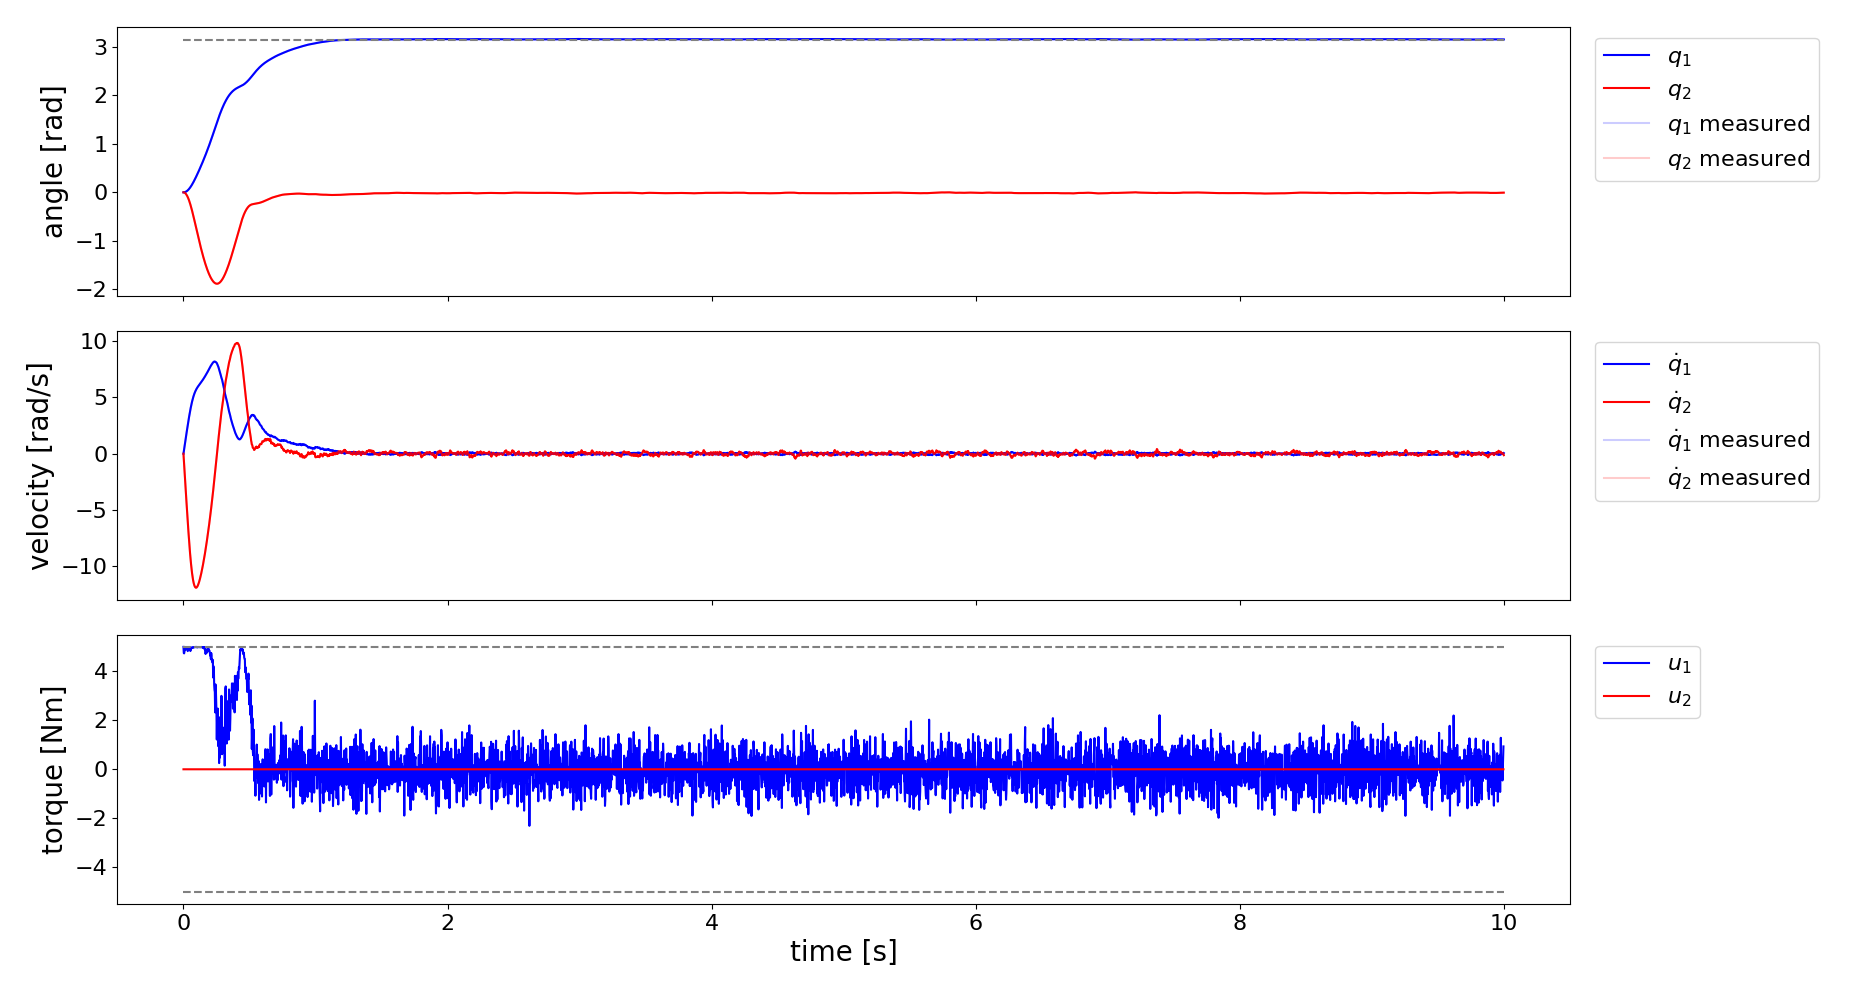
\includegraphics[width=0.9\textwidth]{figures/simulation_result/pendubot_self_stablization.png}} % First image
    \caption{Self stabilization of pendubot in simulation}
    \label{fig:pendubot_self_stablization}
\end{figure}

Self-stabilization behavior has been observed in the acrobot setup as well. However, no consistent pattern has yet been identified as to the specific conditions under which the training yields a self-stabilizing agent. Fortunately, the same agent discussed in Section 4.3.2 exhibited a degree of self-stabilization, which is depicted in the figure that follows. In the absence of a LQR controller, the RL-based controller was compelled to devise its own stabilization strategy. As illustrated in the graph, a relatively stable period commences at approximately 4 seconds, during which the system state exhibits prolonged fluctuations around the upright position. This occurs as the controller continuously corrects any deviation from the desired state. Although the stabilization provided by the RL-based controller is less smooth than that of the LQR-based controller, the inclination towards self-stabilization is distinctly apparent.

\begin{figure}[H]
    \centering
    \fbox{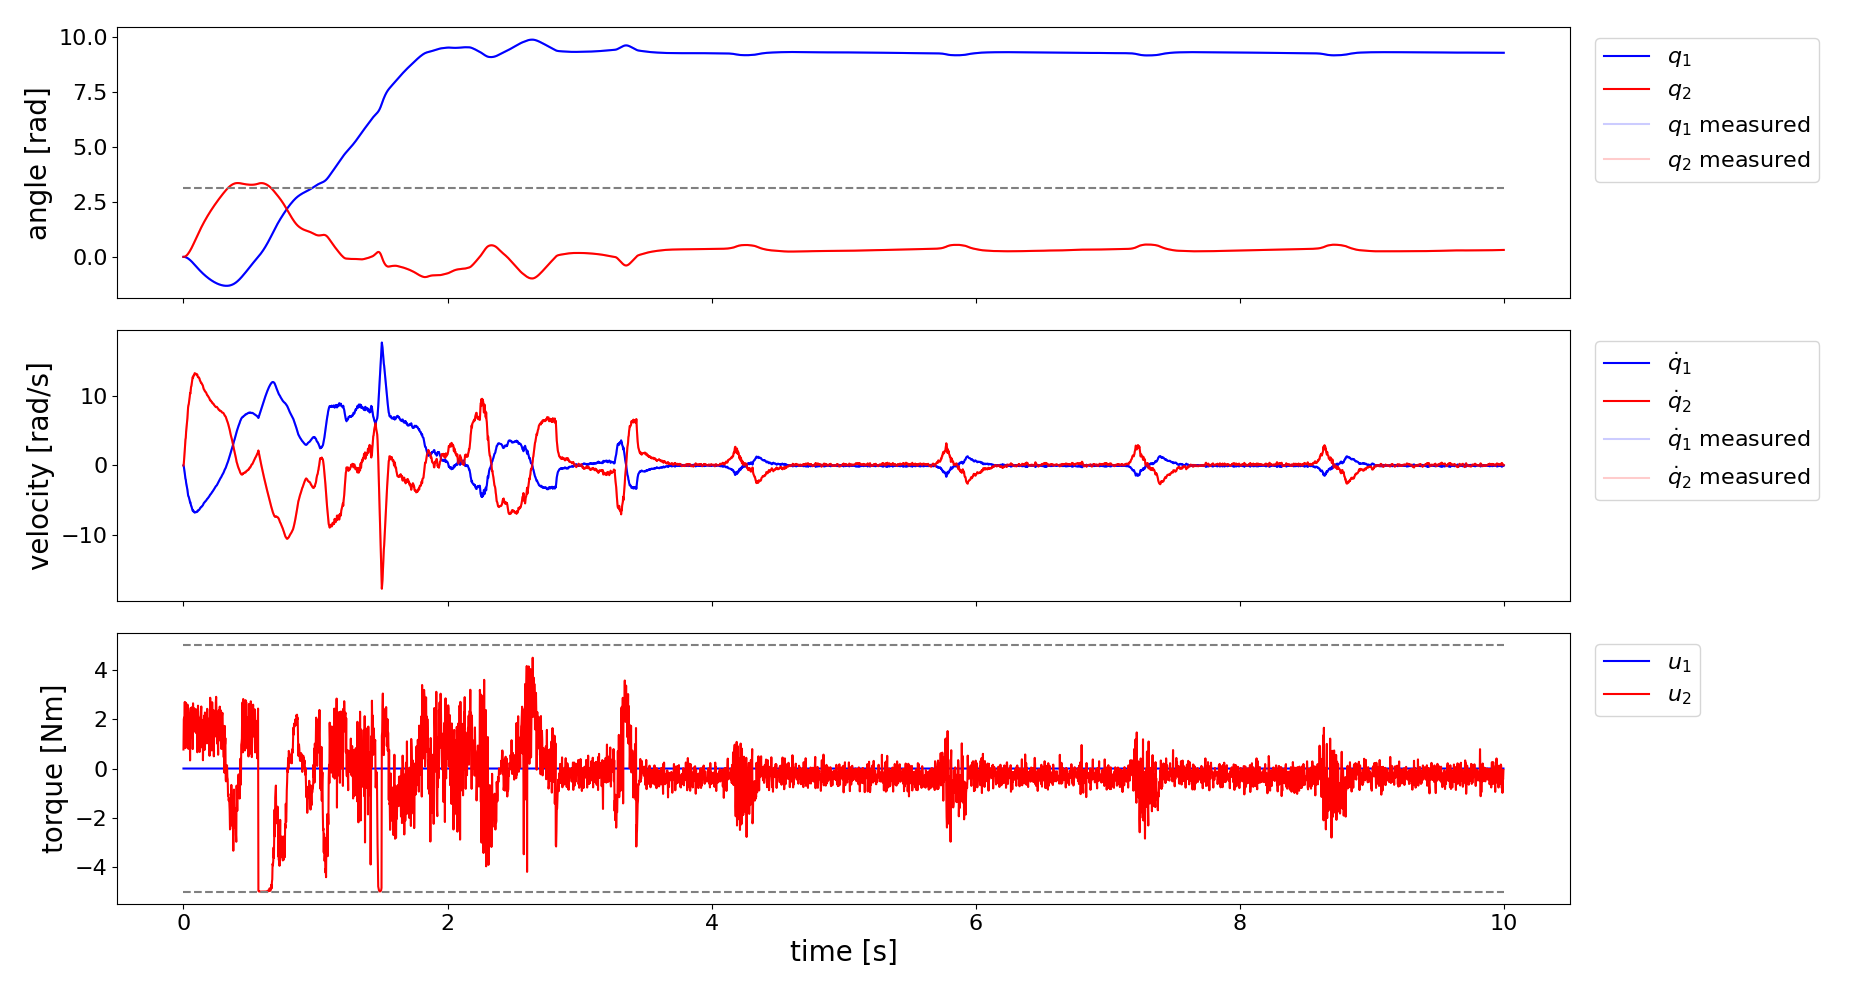
\includegraphics[width=0.9\textwidth]{figures/simulation_result/acrobot_self_stablization.png}} % First image
    \caption{Self stabilization of acrobot in simulation}
    \label{fig:acrobot_self_stablization}
\end{figure}

\cleardoublepage
